%---------- Quinto Capítulo: Resultados ----------

\chapter{Resultados} %5 --- 10 pags

Com o conjunto de ferramentas desenvolvidos neste projeto aliado a uma base de vídeos originais é possível produzir e avaliar uma nova e diversificada base com vídeos degradados em qualidade e quantitade variável.
Neste Capítulo serão verificados os resultados obtidos a partir do processamento de vídeos efuados por estas ferramentas. Primeiramente uma avaliação subjetiva das ferramentas de degradação utilizando diversas amostras retiradas de um vídeo da base. A seguir é feita a validação dos resultados obtidos pela ferramenta de métricas objetivas, tomando como base (base do wyllian!!).
Por fim é feita uma análise das notas de avaliação objetivas buscando mensurar o impacto que determinadas degradações podem ter sobre um conjunto de vídeos com características diferentes.

\section{Validação das Ferramentas de Artefatos}

Foram efetuados diversos processos de degradação sobre o vídeo !!! empregando diferentes paramêtros a cada processamento e para cada ferramenta, buscando identificar visualmente e os artefatos produzidos e determinar sua semelhanca com os vistos em situações reais.

A primeira ferramenta a ser avaliada é a \emph{block}.
Para a avaliação foram gerados 14 vídeos onde é efetuado o processo de blocagem, com blocos 8x8, de forma integral --- para todos os blocos em todos os quadros. A cada novo vídeo gerado foram eliminadas de forma cumulativa diagonais na matriz resultante da transformação DCT, partindo da diagonal mais inferior, até que no último vídeo restasse somente a componente DC da transformada. 
Na Figura \ref{fig:blockbus} são apresentados recortes de 160 por 160 \emph{pixels} a partir da posição 64x160 retirados do frame de número 60 de cada um dos 14 vídeos obtidos, sendo que o primeiro recorte foi obtido do vídeo original.

Observando os recortes com cautela é possível notar degradações extremamente sutis a partir do recorte \emph{07}, verificadas com mais facilidade nos arredores da publicidade na lateral do ônibus.No recorte de número \emph{10} as regiões de alta frequência da imagem denunciam degradações mais acentuadas, e no \emph{11} já não é mais possível identificar o que está escrito na placa de publicidade, embora ainda seja razoavél identificar a cena da imagem.
Nos três recortes seguintes o efeito de blocagem passa a tomar conta da imagem e apenas objetos de grande escala passam a ser identificávies, sendo que no recorte de número \emph{14} até mesmo a identificação da cena fica prejudicada.

\begin{figure}[!htb]
	\centering
	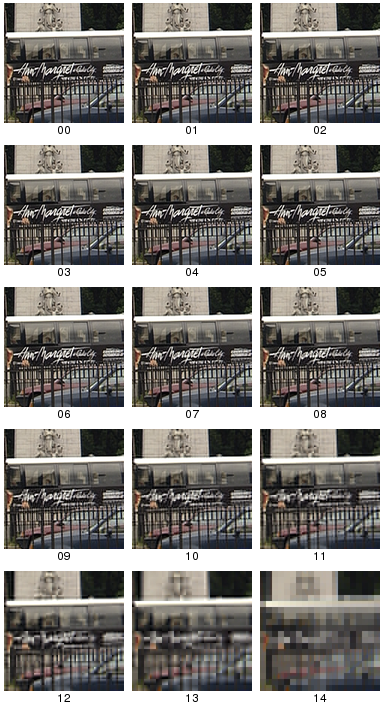
\includegraphics[width=0.8\textwidth]{./imgs/blockbus.png}
	\caption{Sequência de degradações eliminando gradativamente diagonais da DCT.}
	\label{fig:blockbus}
	\fonte{Autoria Própria.}
\end{figure}

\begin{figure}[!htb]
	\centering
	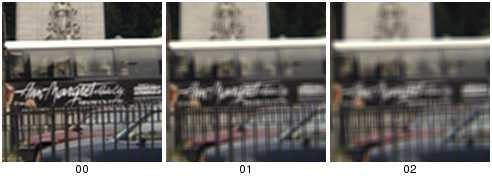
\includegraphics[width=0.9\textwidth]{./imgs/bluraverage.png}
	\caption{.}
	\label{fig:bluraverage}
	\fonte{Autoria Própria.}
\end{figure}

\begin{figure}[!htb]
	\centering
	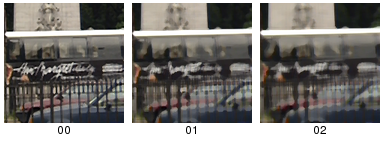
\includegraphics[width=0.9\textwidth]{./imgs/blurmedian.png}
	\caption{.}
	\label{fig:blurmedian}
	\fonte{Autoria Própria.}
\end{figure}

\begin{figure}[!htb]
	\centering
	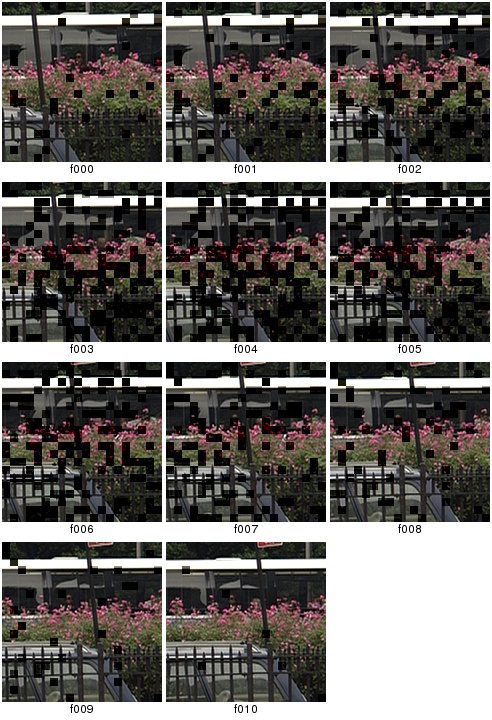
\includegraphics[width=0.7\textwidth]{./imgs/busraffle.png}
	\caption{.}
	\label{fig:busraffle}
	\fonte{Autoria Própria.}
\end{figure}

\begin{figure}[!htb]
	\centering
	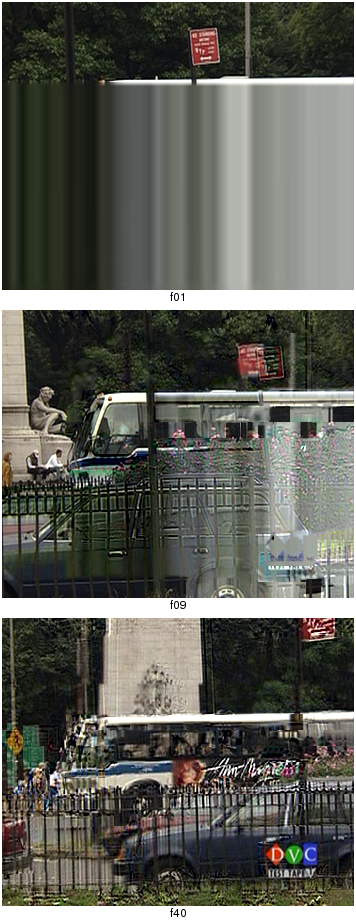
\includegraphics[height=0.9\textheight]{./imgs/netsimresult.png}
	\caption{.}
	\label{fig:netsim}
	\fonte{Autoria Própria.}
\end{figure}

\section{Validação da Ferramenta de Métricas}

\section{Análise de Impacto Sobre Métricas Objetivas}

\section{Resumo e Conclusão do Capítulo}
